\documentclass{beamer}
\mode<presentation>
\usetheme{CambridgeUS}
\usepackage[russian]{babel}
\usepackage[utf8]{inputenc}
\usepackage[T2A]{fontenc}
\usepackage{sansmathaccent}

\usepackage{verbatim}
\usepackage{alltt}

\pdfmapfile{+sansmathaccent.map}
\title[Уровень поверхности]{Уровень поверхности}
\author{Наумов Д.А., доц. каф. КТ}
\date[21.10.2020] {Компьютерная графика и проектирование графических интерфейсов, 2020}

\begin{document}

%ТИТУЛЬНЫЙ СЛАЙД
\begin{frame}
  \titlepage
\end{frame}
  
%СОДЕРЖАНИЕ ЛЕКЦИИ
<<<<<<< HEAD
\begin{frame}
  \frametitle{Содержание лекции}
  \tableofcontents  
\end{frame}
=======
%\begin{frame}
%  \frametitle{Содержание лекции}
%  \tableofcontents  
%\end{frame}
>>>>>>> 939dc34fb518ba07b2790ade3ea3ecf88946e208

\section{Уровень поверхности}
  
\begin{frame}[t]
	\begin{block}{Уровень поверхности}
		визуальное представлениее логического порядка элементов, образующих компоновку сайта. 
	\end{block}
	\begin{figure}[h]
		\centering
		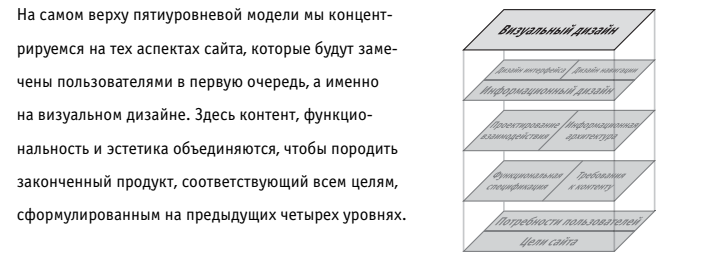
\includegraphics[scale=0.5]{images/lec05-pic01.png}
	\end{figure}
	\begin{itemize}
		\item Насколько эффективно дизайн поддерживает цели, определенные на каждом из нижележащих уровней? 
		\item Не подрывает ли внешний вид сайта его структуру, размывая различия между архитектурными компонентами и делая их неоднозначными?
	\end{itemize}
\end{frame} 

\begin{frame}[t]{Следование за взгядом}
	\begin{itemize}
		\item Куда в первую очередь направляется взгляд? 
		\item Какой элемент дизайна первым притягивает внимание пользователя? 
		\item Направлено ли оно на что-то важное для стратегических целей сайта или первый объект, попадающий в поле зрения, отвлекает пользователя от его (или ваших) целей?
	\end{itemize}
\end{frame}

<<<<<<< HEAD
\begin{frame}[t]{Следование за взгядом}
=======
\begin{frame}[t]
>>>>>>> 939dc34fb518ba07b2790ade3ea3ecf88946e208
	\begin{figure}[h]
		\centering
		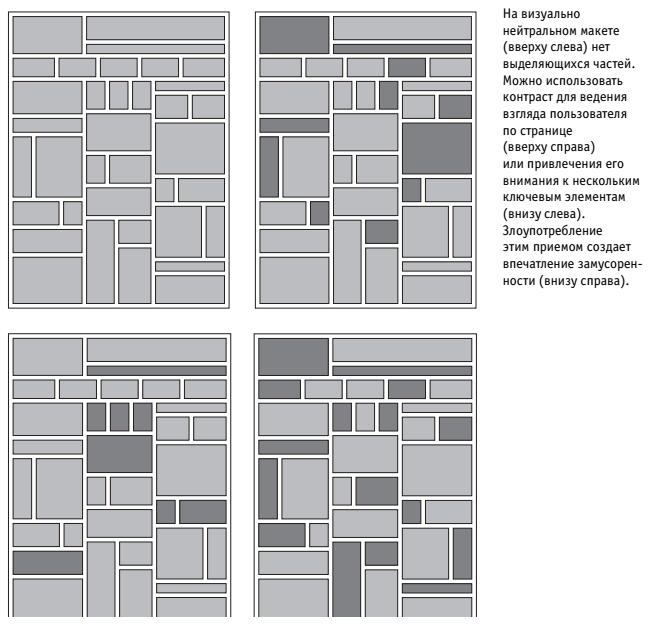
\includegraphics[scale=0.5]{images/lec05-pic02.png}
	\end{figure}
\end{frame}  

\begin{frame}[t]{Контраст и единообразие}
	\begin{itemize}
		\item В визуальном дизайне основным инструментом привлечения внимания пользователя является \textbf{контраст}.

		\item Единообразие в дизайне существенно помогает выстроить эффективную коммуникацию с пользователями, не запутывая и не перегружая их.

		\item Макетная сетка – один из приемов, заимствованных из полиграфии и успешно перенесенных во Всемирную паутину. 

		\item При этом подходе единообразие дизайна достигается использованием <<шаблона макета>> для создания различных вариантов компоновки.
	\end{itemize}
\end{frame}

<<<<<<< HEAD
\begin{frame}[t]{Сетка}
	\begin{figure}[h]
		\centering
		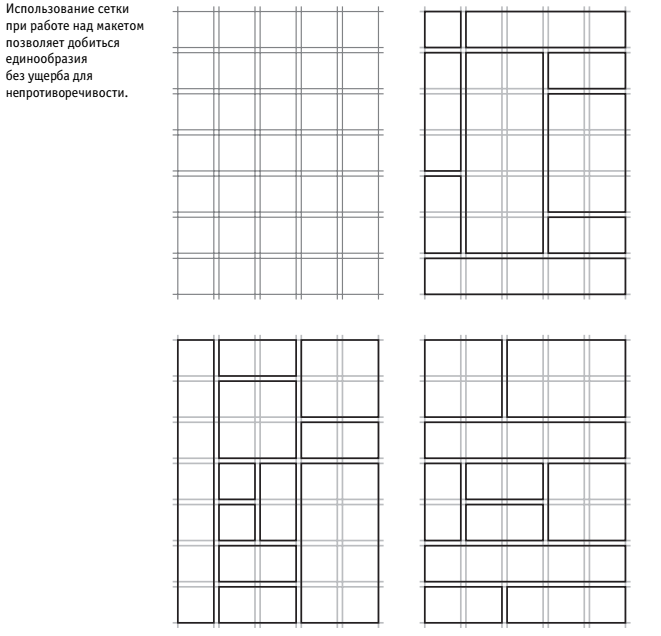
\includegraphics[scale=0.4]{images/lec05-pic03.png}
=======
\begin{frame}[t]
	\begin{figure}[h]
		\centering
		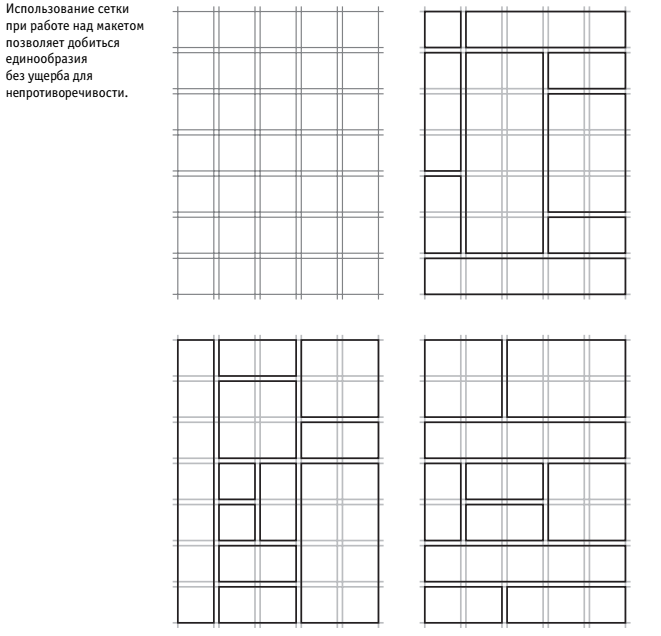
\includegraphics[scale=0.5]{images/lec05-pic03.png}
>>>>>>> 939dc34fb518ba07b2790ade3ea3ecf88946e208
	\end{figure}
\end{frame}  

\begin{frame}[t]{Внутренняя и внешняя согласованность}
	Проблемы с согласованностью визуального дизайна:
	\begin{itemize}
		\item внутренние противоречия, возникающие из-за применения разных подходов к дизайну различных частей сайта;
		\item внешние противоречия, при которых сайт отражает иной подход к дизайну по сравнению с остальной продукцией компании.
	\end{itemize}
<<<<<<< HEAD
	\textbf{Цвет} - один из самых эффективных способов передачи идентичности бренда.
	
	Основные цвета бренда обычно являются частью более широкой цветовой палитры, применяемой во всех материалах компании. 

	Цвета в стандартной палитре специально подбираются так, чтобы они создавали общий эффект, не конкурируя и дополняя друг друга.
\end{frame}

\begin{frame}[t]{Внутренняя и внешняя согласованность}
Типографика, то есть использование шрифтов разного рисунка и размера для создания определенного визуального стиля, настолько важна для идентичности бренда, что некоторые компании заказали для себя разработку специальных шрифтов. 

Принципы эффективного использования шрифтов практически те же, что и для остальных аспектов визуального дизайна: 
не применяйте похожие, но неидентичные шрифты. 
Используйте разные шрифты только для подчеркивания отличий в видах информации, которую вы передаете.
Обеспечьте достаточный контраст между шрифтами, чтобы привлечь внимание пользователя, но не перегружайте дизайн чрезмерным разнообразием шрифтов.
=======
	\textbf{Цвет} - один из самых эффективных способов передачи идентичности бренда.	
	~
	Основные цвета бренда обычно являются частью более широкой цветовой палитры, применяемой во всех материалах компании. 
	~
	Цвета в стандартной палитре специально подбираются так, чтобы они создавали общий эффект, не конкурируя и дополняя друг друга.
\end{frame}

\begin{frame}[t]
	\begin{figure}[h]
		\centering
		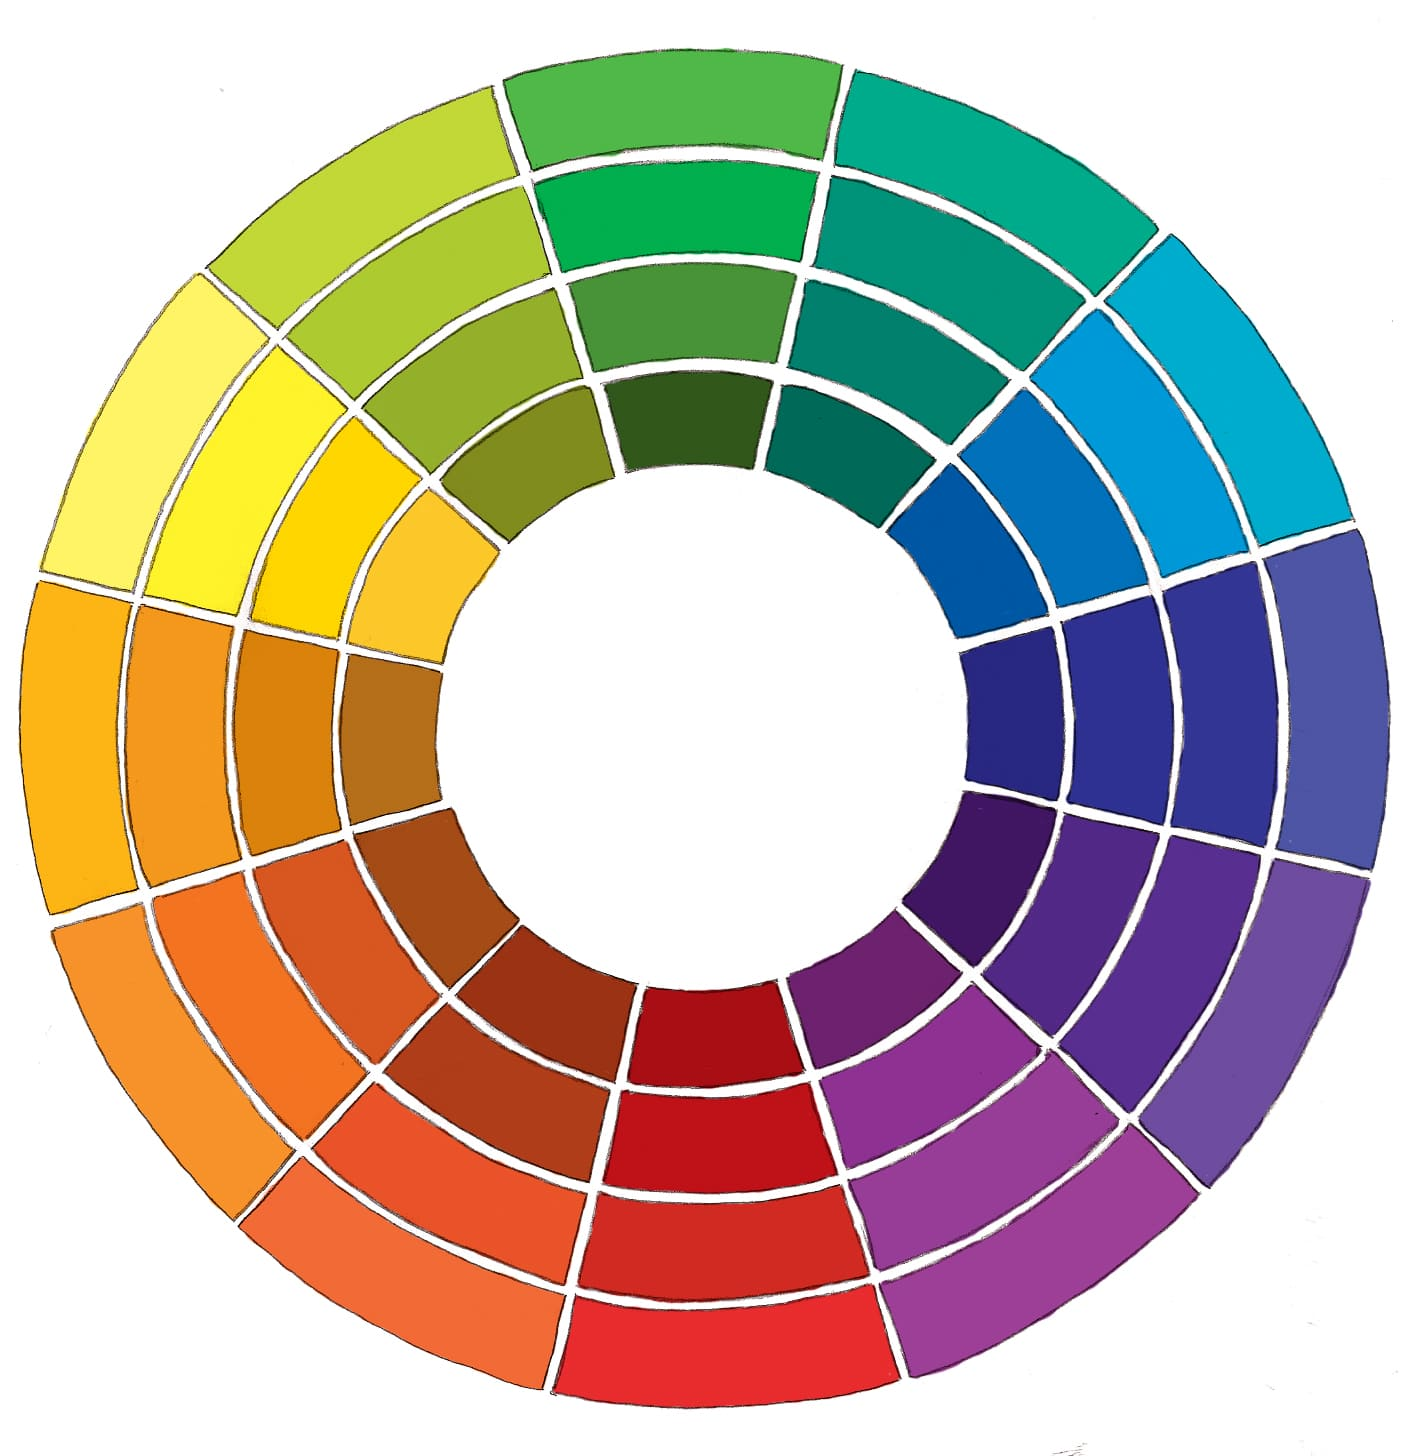
\includegraphics[scale=0.15]{images/color.jpg}
	\end{figure}
\end{frame}  

\begin{frame}[t]{Измерения шрифта}
	\begin{figure}[h]
		\centering
		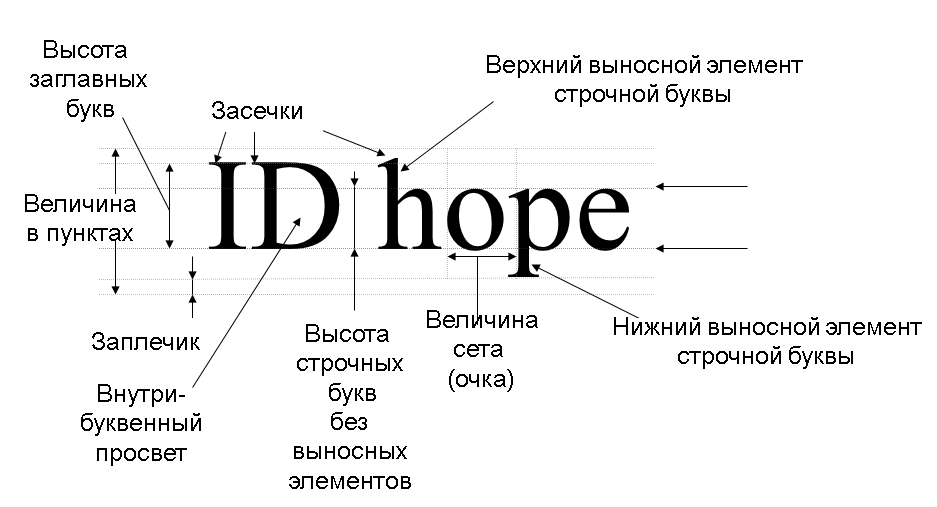
\includegraphics[scale=0.5]{images/lec05-pic05.png}
	\end{figure}
\end{frame}  

\begin{frame}[t]{Начертания шрифта}
	\begin{figure}[h]
		\centering
		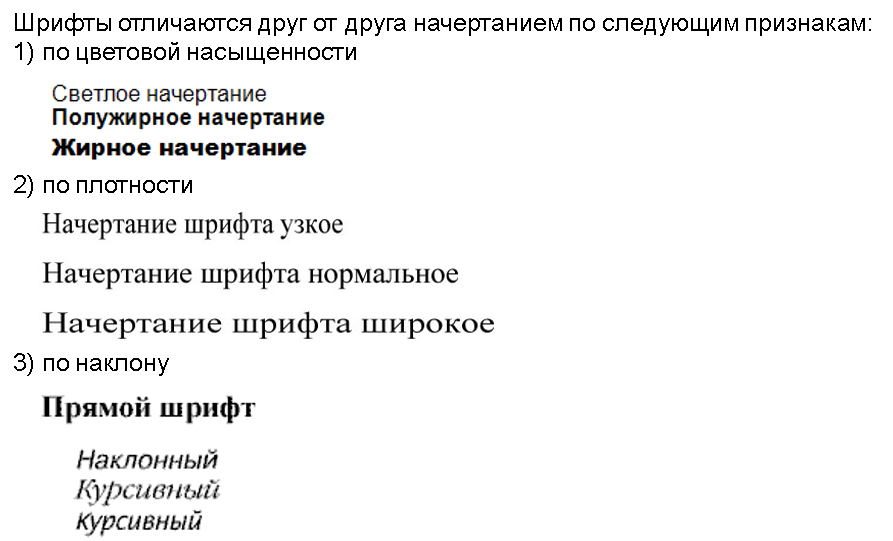
\includegraphics[scale=0.5]{images/lec05-pic06.png}
	\end{figure}
\end{frame}  

\begin{frame}[t]{Шрифты с засечками (serif)}
	\begin{figure}[h]
		\centering
		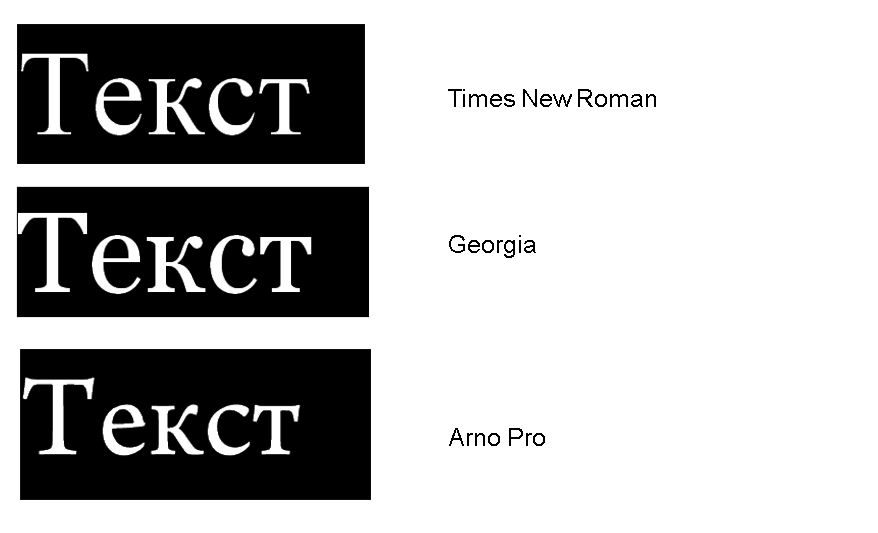
\includegraphics[scale=0.5]{images/lec05-pic07.png}
	\end{figure}
\end{frame}  

\begin{frame}[t]{Шрифты без засечек (sans serif)}
	\begin{figure}[h]
		\centering
		
\includegraphics[scale=0.5]{images/lec05-pic08.png}
	\end{figure}
\end{frame}  

\begin{frame}[t]{Рукописные шрифты (script)}
	\begin{figure}[h]
		\centering
		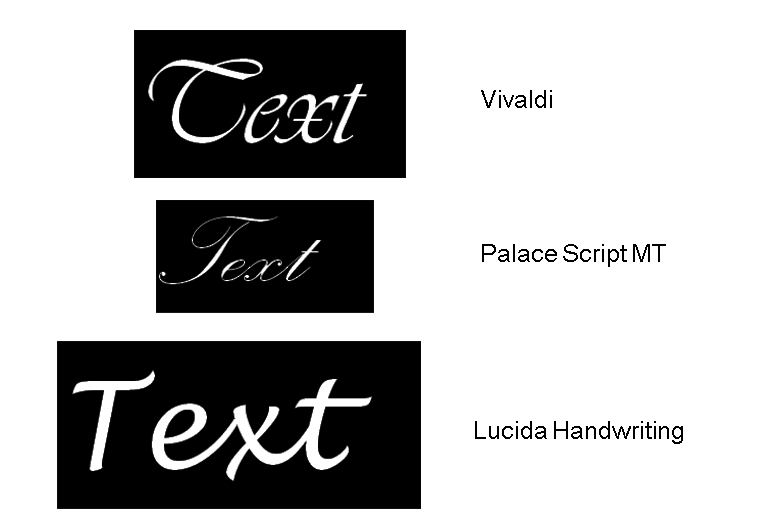
\includegraphics[scale=0.5]{images/lec05-pic09.png}
	\end{figure}
\end{frame}  

\begin{frame}[t]{Декоративные шрифты}
	\begin{figure}[h]
		\centering
		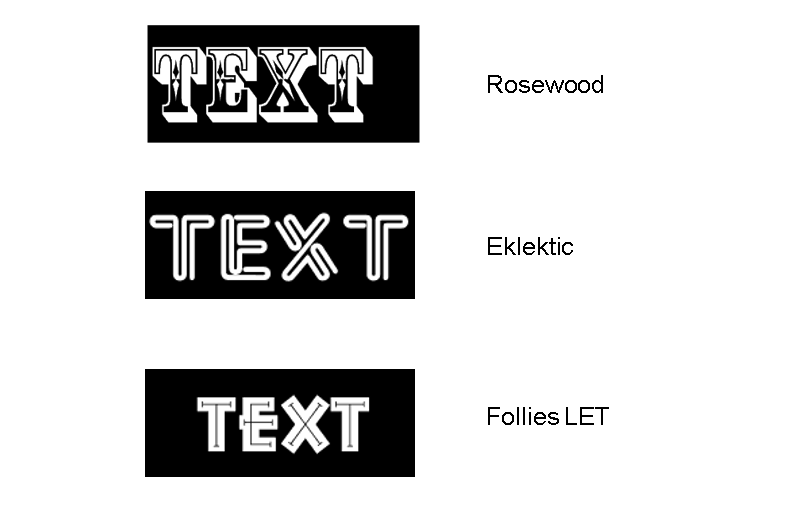
\includegraphics[scale=0.5]{images/lec05-pic10.png}
	\end{figure}
\end{frame}  

\begin{frame}[t]{Внутренняя и внешняя согласованность}
	\textbf{Типографика}, то есть использование шрифтов разного рисунка и размера для создания определенного визуального стиля, настолько важна для идентичности бренда, что некоторые компании заказали для себя разработку специальных шрифтов. 
	~
	Принципы эффективного использования шрифтов: 
	\begin{itemize}
		\item не применяйте похожие, но неидентичные шрифты; 
		\item bспользуйте разные шрифты только для подчеркивания отличий в видах информации, которую вы передаете;
		\item обеспечьте достаточный контраст между шрифтами, чтобы привлечь внимание пользователя;
		\item не перегружайте дизайн чрезмерным разнообразием шрифтов.
	\end{itemize}
	\begin{figure}[h]
		\centering
		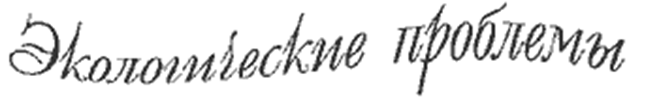
\includegraphics[scale=0.5]{images/lec05-pic11.png}
	\end{figure}	
>>>>>>> 939dc34fb518ba07b2790ade3ea3ecf88946e208
\end{frame}

\begin{frame}[t]{Макет и стиль}
	Визуальный дизайн не обязан в точности совпадать с прототипом страниц – он должен лишь учитывать относительную важность и группировку элементов в том виде, как это представлено на прототипе.
	\begin{figure}[h]
		\centering
		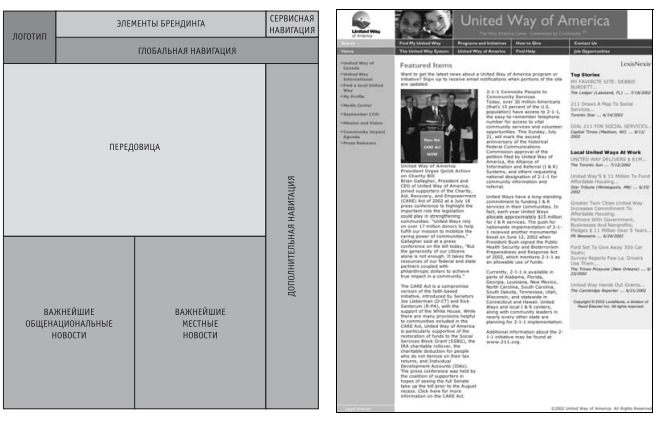
\includegraphics[scale=0.5]{images/lec05-pic04.png}
	\end{figure}
\end{frame} 

\begin{frame}[t]{Что читать дальше}
	\begin{itemize}
		\item Mullet, Kevin and Darrell Sano. Designing Visual Interfaces: Communication Oriented Techniques. Prentice Hall, 1994.
		\item Williams, Robin. The Non-Designer's Design Book. Peachpit, 1994.
	\end{itemize}
\end{frame}

\end{document}
